% begin module cylindrical-shells-ex
\begin{frame}
\begin{example}[$f(x) = 2x^2 - x^3$ Rotated About the $y$-axis]
\begin{columns}
\column{0.6\textwidth}
\only<handout:0| -1>{%
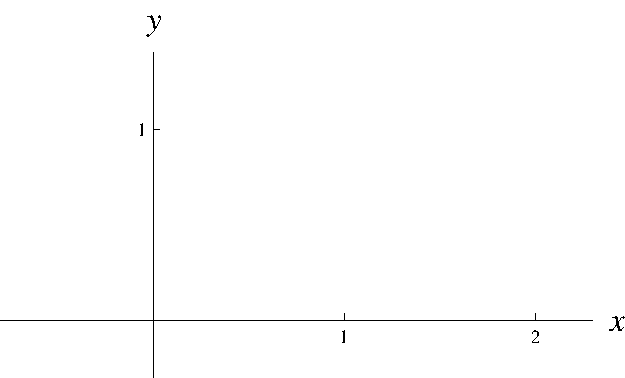
\includegraphics[width=7cm]{volumes/pictures/06-03-exa.pdf} %
}%
\only<handout:0| 2>{%
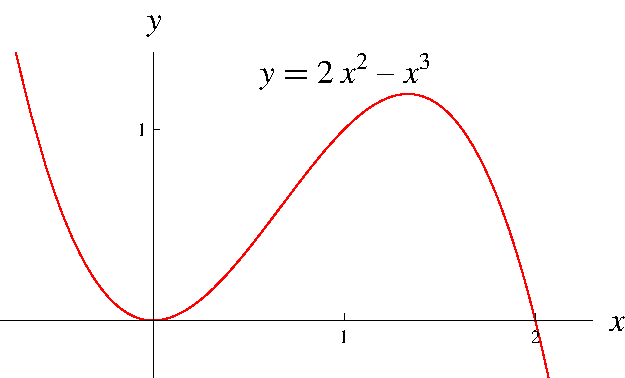
\includegraphics[width=7cm]{volumes/pictures/06-03-exb.pdf} %
}%
\only<handout:0| 3>{%
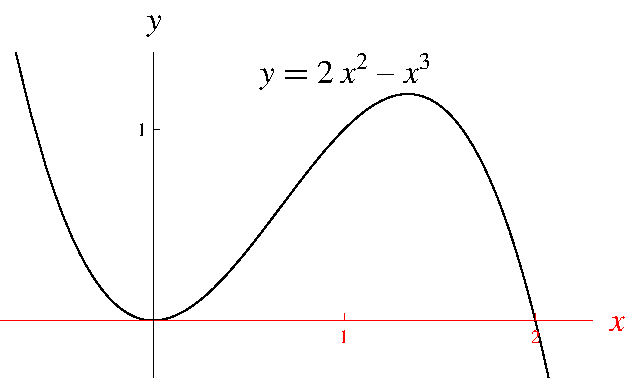
\includegraphics[width=7cm]{volumes/pictures/06-03-exc.pdf} %
}%
\only<handout:0| 4>{%
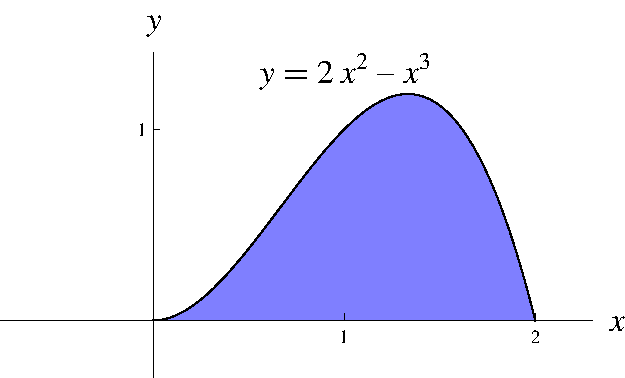
\includegraphics[width=7cm]{volumes/pictures/06-03-exd.pdf} %
}%
\only<5->{%
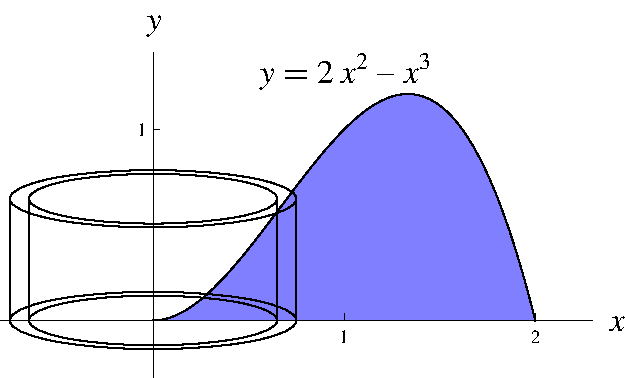
\includegraphics[width=7cm]{volumes/pictures/06-03-exe.pdf} %
}%
\column{0.4\textwidth}
Find the volume of the solid obtained by rotating about the $y$-axis \alert<handout:0| handout:0| 4>{the region bounded by \alert<handout:0| handout:0| 2>{$y = 2x^2 - x^3$} and \alert<handout:0| handout:0| 3>{the $x$-axis}}.
\end{columns}
\begin{eqnarray*}
\uncover<6->{V} & \uncover<6->{ = } & \uncover<6->{\int_0^2(2\pi x)(2x^2 - x^3)\diff x} %\\
  \uncover<7->{ = }  \uncover<7->{2\pi \int_0^2 (\alert<handout:0| 8-9>{2x^3} - \alert<handout:0| 10-11>{x^4})\diff x} \\
 & \uncover<8->{ = } & \uncover<8->{2\pi \left[ \alert<handout:0| 9>{\uncover<9->{\frac{x^4}{2}}} - \alert<handout:0| 11>{\uncover<11->{\frac{x^5}{5}}}\right]_0^2 } %\\
  \uncover<12->{ = }  \uncover<12->{2\pi \left( \frac{16}{2} - \frac{32}{5}\right) } %\\
  \uncover<13->{ = }  \uncover<13->{\frac{16}{5}\pi } \\
\end{eqnarray*}
\end{example}
\end{frame}
% end module cylindrical-shells-ex
